\subsection{Desarrollo teórico}
\label{subsec:desarrollo}
Para comenzar el desarrollo teórico, primero definiremos la geometría de la bobina de manera esquemática para entender bien el sistema con el que trabajamos. De manera descriptiva, lo que tenemos es un cilindro hueco de radio \( r_{cint} \) y altura \( h_c \) sobre el cual enrollaremos un hilo de cobre \textbf{\textit{N}} veces, resultando en un radio exterior \( r_{cext} \). Ligeramente introducido en el cilindro hueco, se encuentra el vástago, que es un cilindro de acero (REFERENCIAR EL ACERO BIEN) de radio \( r_b \) y longitud \( L_b \). La corriente de alimentación será \( i_{dc} \). En la siguiente figura se resume todo en un esquema:

\begin{figure}[H]
    \centering
    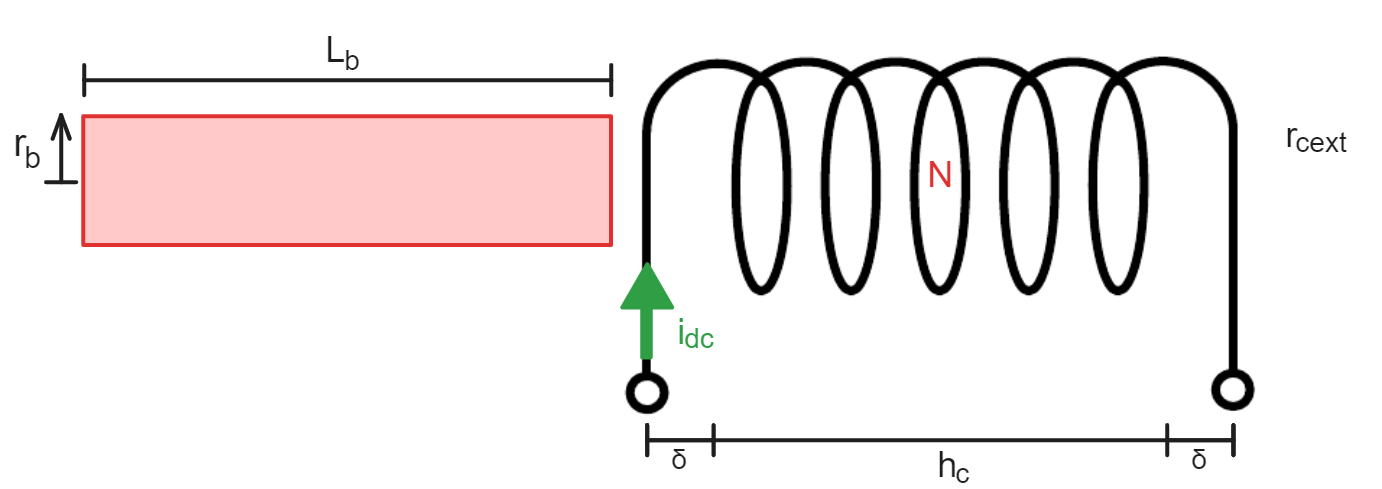
\includegraphics[width=6cm]{FigurasMemoria/fig2esquemaGeom.png}
    \caption{Esquema de la geometría de la bobina. Elaboración propia.}
    \label{fig:3} %Para referenciar -> \ref{fig:figNum}
\end{figure}

Antes de empezar con el desarrollo, hay que aclarar que cuando se empezó este proyecto, se partió de una bobina ya hecha, con la que se han realizado todas las pruebas que se pueden ver en los siguientes apartados. Con el propósito de obtener valores numéricos en esta sección para comprobar de manera cualitativa si el modelo tiene sentido, utilizaremos también los datos de la geometría de la bobina de pruebas para calcular el resultado de las ecuaciones obtenidas. Dichos datos son:

\[
L_b=0.096m~~~~r_b=0.003045m
\\~\\
h_c=0.05321m~~~~r_{cext}=0.01064m
\\~\\
i_{dc}=3.5A~~N=500
\]

El desarrollo teórico empezará por buscar el valor de la inducción electromagnética en la barra, ya que con su valor podremos calcular la fuerza utilizando Lorentz (\textbf{COMPROBAR ESTO IGUAL HAY QUE PONER OTRA COSA}). Para ello, aplicaremos la \textbf{ley integral de Àmpere}:

\[
Ni=\oint{\vec{H}\vec{dl}}
\]

Para simplificar los cálculos, vamos a asumir un flujo uniforme en la bobina ya que tan solo en los extremos (\( \delta \)) el flujo magnético se curvará. Con esto, podemos escribir:

\[
Ni=Hh_c\to H=\frac{Ni_{dc}}{h_c}
\]

Buscamos ahora una expresión para la densidad de flujo:

\[
B=\mu_0\mu_r H=\mu_0\mu_r\frac{Ni_{dc}}{h_c}
\]